
%\documentclass[a4paper,11pt,twoside]{ThesisStyle}
\documentclass[a4paper,11pt,twoside]{article}




\date{\today}
\usepackage{amsmath,amssymb}             % AMS Math
% \usepackage[french]{babel}
\usepackage[latin1]{inputenc}
\usepackage[OT1]{fontenc}
\usepackage[left=2.7cm,right=1.7cm,top=1.6cm,bottom=1.6cm,includefoot,includehead,headheight=13.6pt]{geometry}
\usepackage{setspace}
\usepackage{epigraph}
\usepackage{lineno}


%\usepackage{arev}
%\usepackage[bitstream-charter]{mathdesign}
%\usepackage[urw-garamond]{mathdesign}
%\usepackage[sfmath]{kpfonts} %% sfmath option only to make math in sans serif. Probablye only for use when base font is sans serif.
%\renewcommand*\familydefault{\sfdefault} %% Only if the base font of the document is to be sans serif
\usepackage[sc]{mathpazo}
\linespread{1.05}   
\usepackage[T1]{fontenc}



% Table of contents for each chapter

\usepackage[nottoc, notlof, notlot]{tocbibind}
\usepackage{minitoc}
\setcounter{minitocdepth}{2}
\mtcindent=15pt
% Use \minitoc where to put a table of contents

\usepackage{aecompl}

% Glossary / list of abbreviations

\usepackage[intoc]{nomencl}
\renewcommand{\nomname}{List of Abbreviations}

\makenomenclature

% My pdf code

\usepackage{graphicx,type1cm,eso-pic,color}
\usepackage{lscape}

  \usepackage[pagebackref,hyperindex=true]{hyperref}

%\geometry{letterpaper}
%\graphicspath{{.}{images/}}

% nicer backref links
\renewcommand*{\backref}[1]{}
\renewcommand*{\backrefalt}[4]{%
\ifcase #1 %
(Not cited.)%
\or
(Cited on page~#2.)%
\else
(Cited on pages~#2.)%
\fi}
\renewcommand*{\backrefsep}{, }
\renewcommand*{\backreftwosep}{ and~}
\renewcommand*{\backreflastsep}{ and~}

% Links in pdf
\usepackage{color}
\definecolor{linkcol}{rgb}{0,0,0.4} 
\definecolor{citecol}{rgb}{0.5,0,0} 

% Change this to change the informations included in the pdf file

% See hyperref documentation for information on those parameters

\hypersetup
{
bookmarksopen=true,
pdftitle="",
pdfauthor="", pdfsubject="", %subject of the document
%pdftoolbar=false, % toolbar hidden
pdfmenubar=true, %menubar shown
pdfhighlight=/O, %effect of clicking on a link
colorlinks=true, %couleurs sur les liens hypertextes
pdfpagemode=None, %aucun mode de page
pdfpagelayout=SinglePage, %ouverture en simple page
pdffitwindow=true, %pages ouvertes entierement dans toute la fenetre
linkcolor=linkcol, %couleur des liens hypertextes internes
citecolor=citecol, %couleur des liens pour les citations
urlcolor=linkcol %couleur des liens pour les url
}

% definitions.
% -------------------

\setcounter{secnumdepth}{3}
\setcounter{tocdepth}{2}

% Some useful commands and shortcut for maths:  partial derivative and stuff
\newcommand{\xbp}{$x_{Bj}$}
\newcommand{\xb}{$x_{Bj}~$}
\newcommand{\ptp}{$p_\perp^2$}
\newcommand{\pt}{$p_\perp^2~$}
\newcommand{\dptp}{$\Delta \langle p_\perp^2 \rangle$}
\newcommand{\dpt}{$\Delta \langle p_\perp^2 \rangle ~$}

\brokenpenalty10000\relax

\newcommand{\pd}[2]{\frac{\partial #1}{\partial #2}}
\def\abs{\operatorname{abs}}
\def\argmax{\operatornamewithlimits{arg\,max}}
\def\argmin{\operatornamewithlimits{arg\,min}}
\def\diag{\operatorname{Diag}}
\newcommand{\eqRef}[1]{(\ref{#1})}

\usepackage{rotating}                    % Sideways of figures & tables
%\usepackage{bibunits}
%\usepackage[sectionbib]{chapterbib}          % Cross-reference package (Natural BiB)
%\usepackage{natbib}                  % Put References at the end of each chapter
                                         % Do not put 'sectionbib' option here.
                                         % Sectionbib option in 'natbib' will do.
\usepackage{fancyhdr}                    % Fancy Header and Footer

% \usepackage{txfonts}                     % Public Times New Roman text & math font
  
%%% Fancy Header %%%%%%%%%%%%%%%%%%%%%%%%%%%%%%%%%%%%%%%%%%%%%%%%%%%%%%%%%%%%%%%%%%
% Fancy Header Style Options

\pagestyle{fancy}                       % Sets fancy header and footer
\fancyfoot{}                            % Delete current footer settings

%\renewcommand{\chaptermark}[1]{         % Lower Case Chapter marker style
%  \markboth{\chaptername\ \thechapter.\ #1}}{}} %

%\renewcommand{\sectionmark}[1]{         % Lower case Section marker style
%  \markright{\thesection.\ #1}}         %

\fancyhead[LE,RO]{\bfseries\thepage}    % Page number (boldface) in left on even
% pages and right on odd pages
\fancyhead[RE]{\bfseries\nouppercase{\leftmark}}      % Chapter in the right on even pages
\fancyhead[LO]{\bfseries\nouppercase{\rightmark}}     % Section in the left on odd pages

\let\headruleORIG\headrule
\renewcommand{\headrule}{\color{black} \headruleORIG}
\renewcommand{\headrulewidth}{1.0pt}
\usepackage{colortbl}
\arrayrulecolor{black}

\fancypagestyle{plain}{
  \fancyhead{}
  \fancyfoot{}
  \renewcommand{\headrulewidth}{0pt}
}

%\usepackage{algorithm}
%\usepackage[noend]{algorithmic}

%%% Clear Header %%%%%%%%%%%%%%%%%%%%%%%%%%%%%%%%%%%%%%%%%%%%%%%%%%%%%%%%%%%%%%%%%%
% Clear Header Style on the Last Empty Odd pages
\makeatletter

\def\cleardoublepage{\clearpage\if@twoside \ifodd\c@page\else%
  \hbox{}%
  \thispagestyle{empty}%              % Empty header styles
  \newpage%
  \if@twocolumn\hbox{}\newpage\fi\fi\fi}

\makeatother
 
%%%%%%%%%%%%%%%%%%%%%%%%%%%%%%%%%%%%%%%%%%%%%%%%%%%%%%%%%%%%%%%%%%%%%%%%%%%%%%% 
% Prints your review date and 'Draft Version' (From Josullvn, CS, CMU)
\newcommand{\reviewtimetoday}[2]{\special{!userdict begin
    /bop-hook{gsave 20 710 translate 45 rotate 0.8 setgray
      /Times-Roman findfont 12 scalefont setfont 0 0   moveto (#1) show
      0 -12 moveto (#2) show grestore}def end}}
% You can turn on or off this option.
% \reviewtimetoday{\today}{Draft Version}
%%%%%%%%%%%%%%%%%%%%%%%%%%%%%%%%%%%%%%%%%%%%%%%%%%%%%%%%%%%%%%%%%%%%%%%%%%%%%%% 

\newenvironment{maxime}[1]
{
\vspace*{0cm}
\hfill
\begin{minipage}{0.5\textwidth}%
%\rule[0.5ex]{\textwidth}{0.1mm}\\%
\hrulefill $\:$ {\bf #1}\\
%\vspace*{-0.25cm}
\it 
}%
{%

\hrulefill
\vspace*{0.5cm}%
\end{minipage}
}

\let\minitocORIG\minitoc
\renewcommand{\minitoc}{\minitocORIG \vspace{1.5em}}

\usepackage{multirow}
%\usepackage{slashbox}

\newenvironment{bulletList}%
{ \begin{list}%
	{$\bullet$}%
	{\setlength{\labelwidth}{25pt}%
	 \setlength{\leftmargin}{30pt}%
	 \setlength{\itemsep}{\parsep}}}%
{ \end{list} }

\newtheorem{definition}{D�finition}
\renewcommand{\epsilon}{\varepsilon}

% centered page environment

\newenvironment{vcenterpage}
{\newpage\vspace*{\fill}\thispagestyle{empty}\renewcommand{\headrulewidth}{0pt}}
{\vspace*{\fill}}


\begin{document}


\section*{Reviewers' comments (Oct. 11th, 2017)}

Reviewer \#1: Dear Author, please find here a list of comments from my side.

Summary: the article describes the layout, operation and performances of a 
Radial Time Projection Chamber with the electron amplification stage provided 
by three layers of GEM. The main novelty is the application of the electron 
multiplier for the amplification stage in a TPC on a semi-cylindrical shaped 
plane. The detector, originally built for the BoNuS experiment, is in fact 
formed by two semi-cylindrically shaped halves connected together, with the 
axis coincident with the beam line.\\
 
The detector was implemented to measure DVCS of electrons on different light 
nuclei and the performances were evaluated on electron-$^4$He elastic 
scattering runs.\\

Chapter 1 describes the CLAS@JLab detector, inside which the RTPC was installed 
and took data. Chapter 2 focuses on the RTPC mechanical and electrical layout.  
From inner to outer, there are: the $^4$He gas target, a $^4$He gas gap, the 
actual time projection chamber. The time projection chamber is a 200~mm long 
detector composed by different gas gaps limited by concentric electrodes around 
the axis: cathode (R= 30~mm), G1(R= 60~mm), G2(R= 63~mm), G3(R= 66~mm), readout 
plane (R= 69~mm). Everything fits inside a 5T solenoidal magnetic field. It 
provides both time and charge measurements. Chapter 3 is a short description of 
the electronics and readout, mainly inherited from ALICE and BoNuS. The 
improvement stands in the higher readout rate capability. Chapter 4 talks about 
calibration of drift velocity, drift paths and energy loss measurements by the 
usage of simulations with MAGBOLTZ and tuning the results on elastic scattering 
data. Chapter 5 concentrates on track finding/fitting procedure and noise 
evaluation and subtraction. Chapter 6 reports on resolution and efficiency from 
the elastic scattering reconstruction of 1 GeV electrons on 4He and Chapter 7 
concludes the paper.\\

The article main points of interest are the followings:

a) The usage of GEMs as avalanche creators inside the time projection chamber.  
As far as I know other TPC with the wires substituted by GEM layers have been 
(or are being) realized, like ALICE TPC upgrade or the FOPI one (proposed for 
PANDA), but in those cases the GEM are planar and on the end plane of the TPC, 
not around the beamline.

b) The shaping of the GEM foils around the target. However, since now a fully 
cylindrical GEM foil has been realized (for the KLOE-2 detector and for the 
next BESIII inner tracker) I would not call these "cylindrical" GEMs, but 
"semi-cylindrical" GEMs to point out the difference (which reflects in the 
construction procedure). Maybe these other experiments using GEMs should be 
mentioned due to the similarities, thought they are successive in time to this 
RTPC construction.\\ 

Concerning the work description, it is mainly exhaustive, but in some points 
there are open questions that I would like to submit to the authors in the 
following.

\newpage
\section*{Chapter by chapter comments}

\begin{enumerate}

\subsection*{Chapter 2}
\item As already said I would not speak of cylindrical GEMs but 
   semi-cylindrical. Moreover, please add the reference to Sauli's paper [11] 
   when speaking the first time about GEM in the text.\\
\textcolor{blue}{cylinderical GEMs-> semi-cylinderical. The reference has been added.} 

\item In my opinion, this chapter should highlight better which are the 
   improvements w.r.t. BoNuS detector to underline the originality of this 
   work. For example, better acceptance? Higher gain? Higher electric 
   stability? Lower material budget? Please quote some old and new values, 
   maybe in a table, to make them evident.\\
\textcolor{red}{To the group: Do we have such a comparison? } 

\item Relevant length and thicknesses of the various elements are reported in 
   the text and in the figure, can you please add also the z position of the 
   target w.r.t the detector? To give the complete information, I would also 
   add the value of the induction gap electric field, which is the only missing 
   field value and the value of the reached amplification gain with the three 
   GEM.\\
\textcolor{blue}{- The target tube is the central z-axis of the detector. The 
text is modified to make it clean.\\}
\textcolor{red}{- Regarding the electric field, it was 2.8 kV/cm in BoNuS, does 
anyone know our exact field in this gap?\\}
\textcolor{blue}{- The gain of such GEM configuration has been studied by 
   CERN's Gas Detector Development Group (Fabio Sauli, Progress with the Gas 
   Electron Multiplier, 2nd Workshop on Advanced Transition Radiation Detectors 
   for Accelerator and Space Applications (Bari, Sept. 4-7, 2003), Nucl. Instr. 
   and Meth. A522(2004)93). The results, see the reference, demonstrate that 
one should not simply add gains to each other for multilayer GEM 
amplifications.  We did not evaluate precisely the overall gain in our chamber, 
so we do not have a value for our RTPC GEM system at this point.}

\item When speaking of low spark rate the reference [12] is quoted, which is 
   the PDG. Maybe it is better to quote more specific studies like the ones by 
   Bachmann et al.\\
\textcolor{blue}{Thanks. It has been replaced.} 

\item line 119: is the Kapton of the GEM foil really 300 mum thick? It is 
   usually very thin, like 50 mum, in order to have low material budget and 
   very high fields.\\
\textcolor{blue}{Sorry typo. It is 50 $mu$m} 

\subsection*{ Chapter 3}
\item The description of the electronics looks to me a little not well 
   organized, like a collection of info from previous descriptions from ALICE 
   and BoNuS. It is a series of details, some of which not really relevant for 
   the good understanding of the work described in the paper. So, I would put 
   only some general info (the number of channels/pad, the number of time 
   samples and their width for each channel and the number of  ADC samples and 
   their width for each channel) with the reference where to find more material 
   and just write explicitly the novelties, such as the fact that the 
   acquisition rate was increased (footnote 2).\\
\textcolor{red}{Raphael, Can you check here?} 

\item Also, I understand that fig. 5 comes from reference [14], updated with 
   the values of the RTPC instead of the ALICE-TPC, but it seems to me that 
   there are some parts of the picture which have to be fixed. I list them 
   here:\\
- why does it say 768 pads?\\
- why 7.6 microsec?\\
- the anode wire e grid make no sense here\\
- why L1 and L2 (trigger levels?) \\
\textcolor{red}{Raphael, Can you check here? } 

\subsection*{ Chapter 4}
	/paragraph 4.1
\item I would really prefer to call it drift "velocity" instead of drift 
   "speed"\\
\textcolor{red}{To the group: We do have radial and azimuthal drift velocities, 
but we measure the average of their sum. } 

\item I don't really understand the procedure to find the drift velocity 
   described here and fig. 7. What is $Nb_{max}$ and $Nb_{max/2}$? Why does 
   $T_{max/2}$ correspond to $Nb_{max/2}$ and why is it used as $T_{max}$? If I 
   make a quick calculation and use $T_{max}$ ~ 65 * 100ns and a drift length 
   of ~ 3cm /cos(23°) ~ 7.5 cm I get a $v_{drift}$ ~ 1.15 cm/microsec << 5 
   cm/microsec which is the average value of drift velocity in drift 
   chambers.\\
The procedure according to me would be:\\
- for each hit associated to a track, whose time information is available, take 
the drift time $t_{drift_{i}}$;\\
- plot the distribution of these $t_{drift_{i}}$;\\
- find the $T_{min}$ = minimum $t_{drift_{i}}$ and $T_{max}$ = maximum 
$t_{drift_{i}}$\\
- compute $delta_{t} = T_{max} - T_{min}$ and extract the drift velocity by 
dividing the track length / $delta_{t}$. Figure 8 would have the $delta_{t}$ 
instead of the $T_{max}$ vs z.\\
Please provide more details on the applied procedure, since I have the open 
questions I wrote before and I could not understand it properly. Moreover, 
please quote the value of the found drift velocity. Is it in accordance with 
the simulations?\\
\textcolor{blue}{ } 

\item Figure 6: why are $T_{min}$ and $T_{max}$ not at the drift gap 
   extremities?\\
   \textcolor{blue}{This is a schematic to illustrate the definitions of 
   $T_{min}$ and $T_{max}$ in a chain of hits. The figure can be modified if 
needed.} 

        /paragraph 4.2

\item line 306: "in one bin" should be explained better. I understood it is the 
   subdivision in bins of the z coordinate, but it was not so obvious at the 
   first reading\\
\textcolor{blue}{The text is cleared} 

\item Has the stability of the drift path been counter checked with simulations 
   varying the field according to the cathode radius variation? How much is the 
   field variation if the radius have some mm of uncertainty?\\
\textcolor{blue}{We did not study this case. } 

        /paragraph 4.3
\item The gain calibration is very quick. I would like more details, e.g. 
   "setting the simulation properly" intends only GEANT4 or also MAGBOLTZ or 
   GARFIELD? Were they used to simulate the drift and avalanche formation of 
   the electrons? And the diffusion from the gas? Was a specific code written 
   to simulate the electronics?\\
\textcolor{blue}{Only GEANT4 simulation was used in performing the gain 
   calibration, where the drift paths are updated in the simulation. The 
   electrons avalanche formation and the gas diffusion are performed though 
GEANT4. We did not implement a detailed description to simulate the 
electronics, but we did apply similar conditions to match the real DAQ, such as 
the rejection of the signals from bad pads and conditions to ensure that each 
pad must have at least 3 consecutive time bins, with ADC values above the 
threshold, 35 ADCs, in order to be recorded. The text is cleared with more 
details. } 

\item line 330: "correction factors" are mentioned. On what? Why haven't only 
   good tracks been used for calibration? Lack of statistics?\\
\textcolor{blue}{Correction factor on the extracted gain for each pad. We used 
the elastic $^4$He tracks as we could calculate the recoil $^4$He kinematics 
from the scattered electron in CLAS to avoid any discrepancy from the RTPC.} 

\item When it says that the pad charge is "compared" to the neighboring ones, 
   what happens next? Is it the noise reduction step described later? If so, 
   please write it. \\
\textcolor{blue}{The gain extraction is following this order: \\
- pass 1: the gain of each pad is defined as the ratio between the mean 
recorded experimental ADCs to the mean simulated ADCs in the same track. Then 
for each pad, the gain ratios were collected from all the identified elastic 
tracks and these gains were fitted by a Landau function to give a
  first pass gain for each pad as the most probable value of the fit.\\
 - pass2: to make sure that the recorded ADCs by a given pad are similar to the 
 recorded ADCs by other pads in the same track, we refined this calibration 
 after the extracted gains were applied to the experimental data. At this step, 
 we compared the mean ADCs of each pad to the mean ADCs of the whole track. 
 This ratio is collected from all the elastic events and a gain correction 
 factor is extracted and applied giving a final gain for each pad.
  } 

\item Figure 11: I don't understand it. How many tracks does the histo contain? 
   If the single pad has 128 channels, how many channels does the single bin 
   contain? Moreover, is the dE calculated on pad by pad basis? In that case, 
   why don't you put just one point in the histo for each pad? What is the mean 
   number of channels or pads fired by one track? Sorry for the list of 
   questions, but I could not understand the figure.\\
   \textcolor{blue}{- It is for only one track (written in the caption).
   - We dont understand your second question. A pad is a channel. Do you mean 
how many pads are fired for a single track? Figure \ref{npd_track} shows the 
number of active pads as a function of the momentum for the collected elastic 
$^4$He tracks.\\
- dE is calculated from the ADCs of the individual pads that read out hits 
  corresponding to the same track. One needed to know the individual step size 
  very precisely to put dEdx from the individual pads, which is not available.  
  - Last question is addressed by figure \ref{npd_track}. The mean value is 
    around 10 pads. }

\begin{figure}[h!]
   \centering
   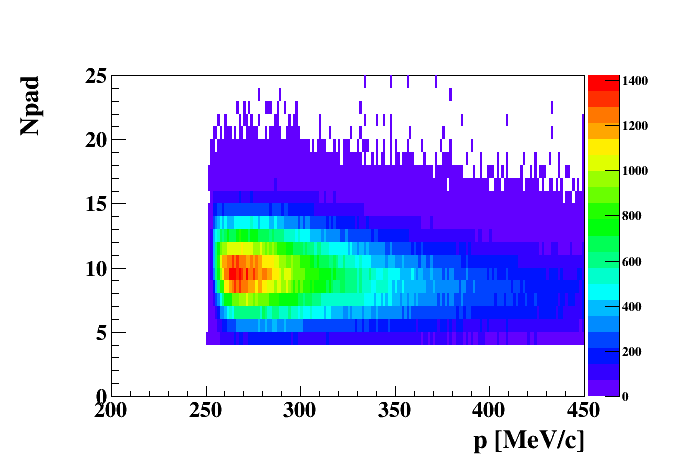
\includegraphics[scale=0.45]{npd_p_elastic.png}
   \caption{The number of active pads versus the measured momentum of the 
   elastic $^4$He tracks. } \label{fig:npd_track}
\end{figure}



\item Figure 12 - please, put it after figure 11. Moreover, please change dEdx 
   to dE/dx on y axis. Why are the left and right pictures so different?  
   Talking about the deuteron band which is present only in the left figure and 
   the smear on the top part of the right picture. \\
\textcolor{red}{- The figures layout will be updated.\\} 
   
\textcolor{blue}{- The y-axis label on figure 12 is updated.\\}
\textcolor{blue}{- Regarding the lower peak in the left module of the RTPC, 
   these events pass all the elastic requirements but for some reasons they 
   have lower ADC values.  They represent around 7\% of all the elastic events.  
   After extended studies, the nature of these particles is not identified yet.  
   We note that this is a global phenomenon in the left module as 94\% of the 
   left module's pads are involved in both some low and high dEdx events. For 
   the calibration procedures, the events with low dEdx were excluded as we do 
not fully understand their nature.} 

\subsection*{ Chapter 5}
        /paragraph 5.1	
     
\item Please detail a little bit more the procedure to remove the oscillatory 
   noise. It says "event by event and channel by channel": if the ADC threshold 
   is passed then a noise level is subtracted? If so, how is it calculated?\\
\textcolor{red}{Nathan, Can you work on it. } 

/paragraph 5.2
\item How was "10.5 mm" cut chosen? is it in xy plane or in 3-dimensions?\\
\textcolor{blue}{The distance between hits are calculated in 3D. This cut has 
been chosen because it enables us to jump longer gaps from dead areas of the 
readout pads without increasing the level of spurious tracks.} 

\item How was the "10 hits" cut chosen? What is the mean number of primary 
   ionization in this gas mixture?\\
   \textcolor{blue}{Figure \ref{fig:nb_hits} shows the number of hits 
   distribution for the collected elastic $^4$He tracks from the 1.2 GeV 
dataset. The mean number of hits is around 135 and the 10 hits cut at the 
reconstruction level is a loose cut to reduce the level of the spurious 
tracks.}

\begin{figure}[h!]
   \centering
   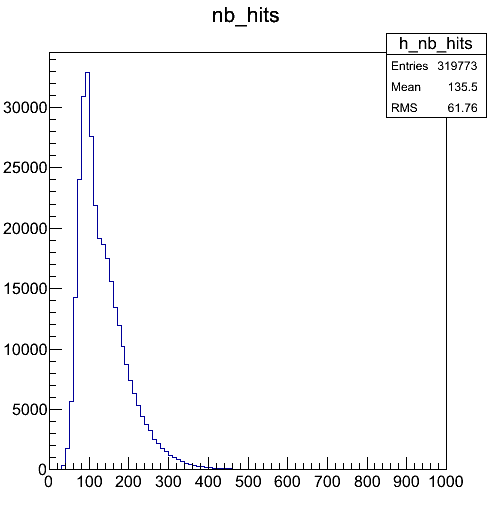
\includegraphics[scale=0.45]{nb_hits.png}
   \caption{the number of hits distribution for the collected elastic $^4$He 
   tracks from the 1.2 GeV dataset.} \label{fig:nb_hits}
\end{figure}


\item < dE/dx > is computed here as corrected Etot divided total track length. 
   Usually the mean dE/dx is computed with the truncated mean of the specific 
   energy losses of each hit. Isn't it possible to compute it like this here? 
   dx for each hit can be (maybe) computed from the difference in the hit 
   times. Sum $dE_{i}$/Sum $dx_{i}$ is not equal to Sum ($dE_{i}/dx_{i}$).\\
\textcolor{blue}{Maybe this would improve our calculations for dEdx by few 
percent, but a precise hits ordering is needed to compute dEdx as you suggest, 
which is not available in our setting.} 

\subsection*{ Chapter 6}

        /paragraph 6.2
\item I understand that efficiency is a ratio between two integrals, each 
   integral being the area of the Gaussian which fits the recoil mass 
   distribution in the inclusive and exclusive case. If so, would it be 
   possible to please draw both fits on the figure 14 and provide the integrals 
   to compute the mean efficiency? If I misunderstood, please comment.\\
\textcolor{red}{Nathan, do you still have the individual integrals? } 

\subsection*{ Chapter 7} 

\item Is it "high rate environment" or "high readout rate"? They are connected, 
   but what is the rate the RTPC underwent during data taking?\\
\textcolor{red}{Can we find such information in the logbook?} 

\item I understand the resolution and efficiency have been evaluated with the 2 
   GeV electrons. Is it foreseen to analyze also the 6 GeV electron runs, which 
   were the actual data taking? Is there an evaluation of the foreseen RTPC 
   performances in that case?\\
\textcolor{blue}{Typically, the elastic reaction is used for such performance 
evaluation. But the elastic cross sections is really small at 6 GeV beam 
energy.} 

\subsection*{ Some general remarks on the layout}

\item I would add to the keywords also GEM or gas electron multipliers or multi 
   pattern gas detectors (it depends on what is available).\\
\textcolor{blue}{Updated} 

\item Please put the units on the axis of every figure, together with the 
   physical quantity. In some figures it is only written in the caption or in 
   the text.\\
\textcolor{blue}{ } 

\item Sometimes to explain the dimension of something something like "250 mm 
   long" (line 67) while some other times "84-mm-long" (on line 83) is written. 
   Please make this uniform in the whole text (I just quoted two examples, but 
   there are more in the text).\\
\textcolor{blue}{Updated everywhere} 

\item In footnote 2, BoNuS is written BONUS and somewhere else in the text also 
   BoNus. Please uniform this to the correct one, which I think is BoNuS.\\
\textcolor{blue}{Updated to BoNuS everywhere} 

\item Please make the bibliography entries uniform: they are not all written 
   with the same layout.\\
\textcolor{blue}{Updated} 

List of in text corrections:

\item line 17: "GeV" --> "GeV/c"\\
\textcolor{blue}{Corrected} 

\item line 26: "nuclei" --> "nucleus"\\
\textcolor{blue}{Corrected} 

\item line 40: "to track" --> "to bend tracks"(since the magnetic field just 
   bends the track and then the detector tracks them)\\
\textcolor{blue}{Added} 

\item line 91: "second gap" --> "second gas gap"\\
\textcolor{blue}{Added} 

\item line 110: "from the GEMs" -->  something like "after they have been 
   multiplied by the GEMs" or "induced in the last gas gap" since the GEM is 
   the amplification system.\\
\textcolor{blue}{Added} 

\item line 131: "axial magnetic field" --> "solenoidal magnetic field"\\
\textcolor{blue}{Replaced} 

\item line 133: "challenge" --> "challenges"\\
\textcolor{blue}{Added} 

\item line 133-134: "radial TPC" it would be better to uniform the way to write 
   it in the whole text (like, "RTPC")\\
\textcolor{blue}{Uniformed} 

\item line 167: "stage" --> "stages"\\
\textcolor{blue}{Corrected} 

\item line 176: "ReadOut" should always be written in the same way (see line 
   168) unless this was specifically written in a different way in the cited 
   articles\\
\textcolor{blue}{Uniformed} 

\item line 208: cm$^{-1}$ . s$^{-1}$ --> cm$^{-1}$ cdot s$^{-1}$ (the dot is 
   not in the center vertically)\\
\textcolor{blue}{Corrected} 

\item line 208 again: "6.067" before it said "6.064", please fix the wrong one
\textcolor{blue}{Corrected. It is 6.064} \\

\item line 263: "2\%" --> I would put "around 2\%"\\
\textcolor{blue}{Added} 

\item line 268: "reconstructions" --> "reconstruction"\\
\textcolor{blue}{Corrected } 

\item line 269: "Paths" --> "Path"\\
\textcolor{blue}{Corrected} 

\item line 308: "codes" --> "code"\\
\textcolor{blue}{Corrected} 

\item line 405: "electron's" --> "electron"\\
\textcolor{blue}{Corrected} 

\item fig14 - caption: "W distribution" --> I would put "recoil mass W 
   distribution"\\
\textcolor{blue}{Added} 

\item table 1: $sigma_{p}$ is actually $sigma_{p/p}$, since it is in 
   percentage\\
\textcolor{blue}{Yes it is. Corrected } 

\item line 432: "Helium-4" --> "4He" (for uniformity, as was written before)\\
\textcolor{blue}{Changed to $^4$He} 

\item line 488: There is an extra "," at the beginning of the item\\
\textcolor{blue}{Cleaned}\\
~\\
\end{enumerate}

The topic of the article is interesting but I would recommend a revision.  
Please I would like the authors to address the questions asked and provide the 
required changes or explain why they think those changes are not 
necessary/correct. Thank you. Best regards.\\


\end{document}
